\documentclass[12pt]{article}
\usepackage[margin=0.1in]{geometry}
\usepackage{arev}
\usepackage{pgfplots}
\usetikzlibrary{calc}
\pgfplotsset{compat=newest}

\begin{document}
\begin{figure}[h]
    \centering
    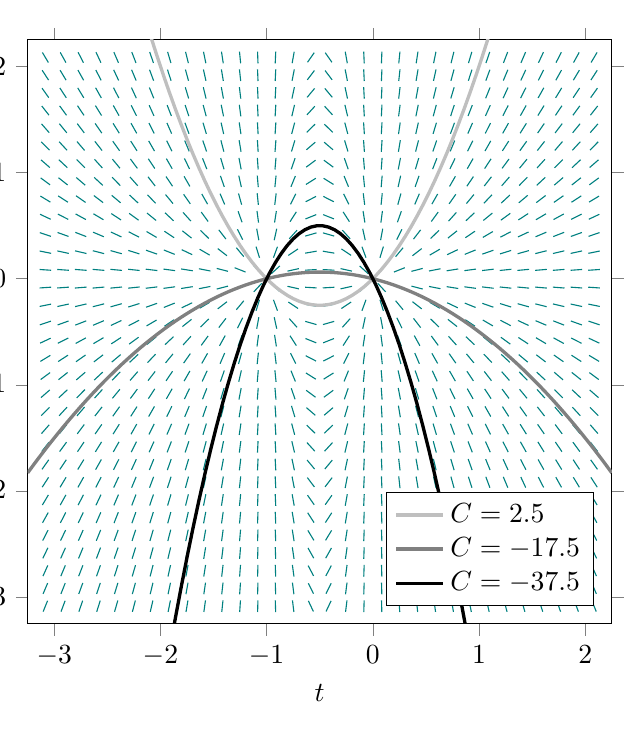
\begin{tikzpicture}[
	    trim axis left, trim axis right, % options to centre correctly
	    declare function={
		dydx(\x,\y) = (2*\x+1)*\y / ((\x)^2+\x); % differential equation
		solution(\x,\c) = \c*(\x^2 + \x); % general solution including constant of integration
	    }
	]
        % axes settings
	\def\width{9cm} \def\height{9cm}
	\def\xmin{-3.25} \def\xmax{2.25}
	\def\ymin{-3.25} \def\ymax{2.25}
        \def\xticks{\xmin+0.25,...,\xmax-0.25}
        \def\yticks{\xticks}

	% actual axis for plotting the solution, must come after slope field to provide proper masking
        \begin{axis}[
		view = {0}{90}, % set camera to point towards x-y plane
	        domain=\xmin:\xmax, xmin=\xmin, xmax=\xmax, ymin=\ymin, ymax=\ymax, xtick=\xticks, ytick=\yticks,
	        xlabel=$t$, ylabel=$w$,
	        tick align=outside,
	        width=\width, height=\height,
	        legend pos=south east, legend cell align={left},
	        axis equal image
	    ]

	    \def\numSlopes{32}
	    \pgfmathsetmacro{\scale}{(\xmax-\xmin)/50}
	    \pgfmathsetmacro{\hx}{(\xmax-\xmin)/(\numSlopes+1)} % +2 to account for the slopes at the domain edge that aren't drawn
	    \pgfmathsetmacro{\hy}{(\ymax-\ymin)/(\numSlopes+1)}
	    \pgfmathsetmacro{\totalSlopes}{\numSlopes^2-1}
	    \pgfplotsinvokeforeach{0,...,\totalSlopes} {
		    \pgfmathparse{mod(#1, \numSlopes))}\edef\i{\pgfmathresult}
		    \pgfmathparse{int(#1 / \numSlopes)}\edef\j{\pgfmathresult}
		    \pgfmathparse{dydx({\hx+\xmin+\i*\hx}, {\hy+\ymin+\j*\hy})}\edef\slope{\pgfmathresult}
		    \pgfmathparse{\scale/sqrt((\slope)^2+1)}\edef\dx{\pgfmathresult}
		    \pgfmathparse{\slope*\dx}\edef\dy{\pgfmathresult}
		    \edef\tmp{\noexpand\draw[teal] ({\hx+\xmin+\i*\hx-\dx/2},{\hy+\ymin+\j*\hy-\slope*\dx/2})--({\hx+\xmin+\i*\hx+\dx/2},{\hy+\ymin+\j*\hy+\slope*\dx/2});}\tmp
	    }

	    % #1: coordinates of node, #2: relative position of node label (can also be angle)
	    \newcommand\labelledPoint[2]{\node[circle, fill, inner sep=2pt, label={[fill=white,distance=1pt,inner sep=1pt]#2:{(#1)}}] at (#1){}}

            % plot initial points and corresponding solution curves
	    \addplot[very thick, black!25, samples=100] {solution(x, 1)};
            % \labelledPoint{0,40}{above right};

	    \addplot[very thick, black!50, samples=100] {solution(x, -0.25)};
            % \labelledPoint{0,20}{above left};

            \addplot[very thick, black!100, samples=100] {solution(x, -2)};
            % \labelledPoint{0,0}{below right};

            % add legend
            \legend{$C=2.5$, $C=-17.5$, $C=-37.5$}
        \end{axis}

    \end{tikzpicture}
    \caption{Slope field of $\frac{\mathrm{d}}{t}=3-0.08w$, with general solution $w(t)=Ce^{-0.08t}+37.5$}
\end{figure}
\end{document}
